\section{The Three Pillars of Learning}
\begin{frame}{The Three Pillars of Learning}
    Every supervised learning algorithm consists of three specific components
    \vspace{1em}
    \begin{enumerate}
        \item \textbf{The Hypothesis (Model)}
        \item \textbf{The Loss Function}
        \item \textbf{The Optimizer}
    \end{enumerate}
    \vspace{1em}
    
\end{frame}

\begin{frame}{1. The Hypothesis (The Model)}
    \begin{itemize}
        \item The mathematical function that maps inputs to predictions.
        \item \textbf{Notation}: $\hat{y} = f(x)$.
        \item It contains \textbf{parameters} (weights) that determine its behavior.
        \item A model is \textbf{"trained"} when these parameters are updated to fit data.
        \item It can be simple (Linear) or complex (Non-linear).
    \end{itemize}
    
    \vspace{0.5em}
    % --- Visual Examples of Models ---
    \begin{columns}[T]
        % 1. Linear Model
        \begin{column}{0.33\textwidth}
            \centering
            \small \textit{Linear Regression}\\[0.3em]
            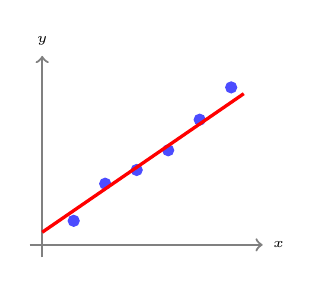
\begin{tikzpicture}[scale=0.8]
                % Axes
                \draw[->, thick, gray] (-0.2,0) -- (3.5,0) node[right, black] {\tiny $x$};
                \draw[->, thick, gray] (0,-0.2) -- (0,3) node[above, black] {\tiny $y$};
                
                % Data points
                \foreach \x in {0.5,1,1.5,2,2.5,3} 
                    \filldraw [blue!70] (\x, 0.7*\x + 0.2 + 0.2*rand) circle (2.5pt);
                
                % Regression line
                \draw [red, very thick] (0,0.2) -- (3.2,2.4);
            \end{tikzpicture}
            
            \vspace{0.3em}
            \small $\hat{y} = wx + b$
        \end{column}
        
        % 2. Decision Tree
        \begin{column}{0.33\textwidth}
            \centering
            \small \textit{Decision Tree}\\[0.3em]
            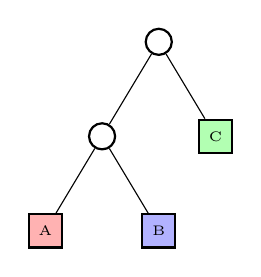
\begin{tikzpicture}[
                scale=0.8,
                level distance=1.5cm,
                sibling distance=1.8cm,
                every node/.style={font=\footnotesize}
            ]
                \node [circle, draw, thick, minimum size=8pt] {}
                    child {node [circle, draw, thick, minimum size=8pt] {}
                        child {node [rectangle, draw, thick, fill=red!30, minimum size=12pt] {\tiny A}}
                        child {node [rectangle, draw, thick, fill=blue!30, minimum size=12pt] {\tiny B}}
                    }
                    child {node [rectangle, draw, thick, fill=green!30, minimum size=12pt] {\tiny C}};
            \end{tikzpicture}
            
            \vspace{1em}
            \small $\hat{y} = \text{tree}(x)$
        \end{column}
        
        % 3. Neural Network
        \begin{column}{0.33\textwidth}
            \centering
            \small \textit{Neural Network}\\[0.3em]
            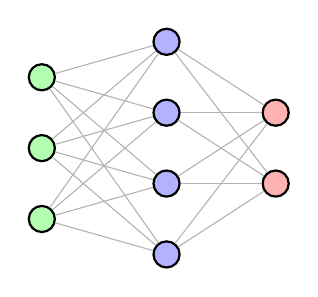
\begin{tikzpicture}[
                scale=0.9,
                x=1.1cm, y=1.0cm,
                every node/.style={circle, draw, thick, minimum size=8pt}
            ]
                % Input Layer (3 neurons)
                \node[fill=green!30] (I1) at (0,3) {};
                \node[fill=green!30] (I2) at (0,2) {};
                \node[fill=green!30] (I3) at (0,1) {};
                
                % Hidden Layer (4 neurons)
                \node[fill=blue!30] (H1) at (1.6,3.5) {};
                \node[fill=blue!30] (H2) at (1.6,2.5) {};
                \node[fill=blue!30] (H3) at (1.6,1.5) {};
                \node[fill=blue!30] (H4) at (1.6,0.5) {};
                
                % Output Layer (2 neurons)
                \node[fill=red!30] (O1) at (3,2.5) {};
                \node[fill=red!30] (O2) at (3,1.5) {};
                
                % Connections - Input to Hidden
                \foreach \i in {1,2,3}
                    \foreach \h in {1,2,3,4}
                        \draw[gray!60, line width=0.4pt] (I\i) -- (H\h);
                
                % Connections - Hidden to Output
                \foreach \h in {1,2,3,4}
                    \foreach \o in {1,2}
                        \draw[gray!60, line width=0.4pt] (H\h) -- (O\o);
            \end{tikzpicture}
            
            \vspace{0.3em}
            \small $\hat{y} = \sigma(W_2\sigma(W_1x))$
        \end{column}
    \end{columns}
\end{frame}

\begin{frame}{2. The Loss Function (The Critic)}
    \begin{columns}[T]
        % Left column: Text content
        \begin{column}{0.48\textwidth}
            \item \textbf{Definition}: A differentiable function $J(\theta)$ that quantifies the \textit{cost} of the model's errors.
            \vspace{0.5em}
            
            \textbf{Goal:} Find model parameters $\theta$ that minimize $J(\theta)$.
            
            \vspace{0.8em}
            \textbf{Common Loss Functions:}
            \begin{itemize}
                \item \textbf{\small Mean Squared Error (MSE)}\\
                (for regression tasks)
                
                \vspace{0.3em}
                \item \textbf{\small Cross-Entropy Loss (Logloss)}\\
                (for classification tasks)
            \end{itemize}
            
            \vspace{0.5em}
            \small\textit{Lower loss = Better model}
            
            \vspace{1em}
            \small{- But how can we minimize the loss?}
        \end{column}
        
        % Right column: Visualization
        \begin{column}{0.48\textwidth}
            \centering
            \textbf{Visualizing Regression Loss}
            
            \vspace{0.5em}
            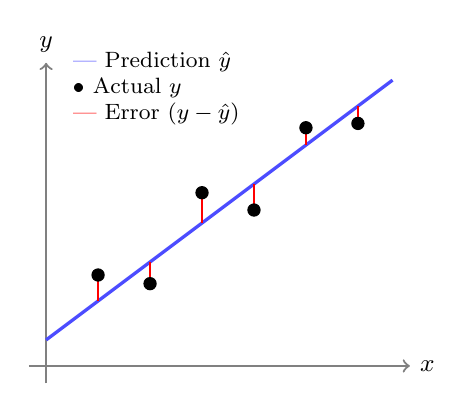
\begin{tikzpicture}[scale=1.1]
                % Axes
                \draw[->, thick, gray] (-0.2,0) -- (4.2,0) node[right, black] {\small $x$};
                \draw[->, thick, gray] (0,-0.2) -- (0,3.5) node[above, black] {\small $y$};
                
                % Regression line
                \draw [blue!70, very thick] (0,0.3) -- (4,3.3);
                
                % Data points and residuals
                \foreach \x/\offset in {0.6/0.3, 1.2/-0.25, 1.8/0.35, 2.4/-0.3, 3.0/0.2, 3.6/-0.2} {
                    \pgfmathsetmacro{\yline}{0.3 + 0.75*\x}
                    \pgfmathsetmacro{\ypoint}{\yline + \offset}
                    \pgfmathsetmacro{\absoffset}{abs(\offset)}
                    
                    % Red vertical line (residual)
                    \draw[red, thick] (\x, \yline) -- (\x, \ypoint);
                    
                    % % Red square showing squared error (correct square)
                    % \fill[red!20, opacity=0.7] (\x, \yline) rectangle ++(\absoffset, \offset);
                    % \draw[red!50, thick] (\x, \yline) rectangle ++(\absoffset, \offset);
                    
                    % Data point
                    \filldraw [black] (\x, \ypoint) circle (2pt);
                }
                
                % Legend
                \node[anchor=west, align=left, font=\footnotesize] at (0.2, 3.2) {
                    \textcolor{blue!70}{—} Prediction $\hat{y}$\\
                    \textcolor{black}{•} Actual $y$\\
                    \textcolor{red}{—} Error $(y-\hat{y})$
                };
            \end{tikzpicture}
            
            \vspace{0.5em}
            \small\textit{The loss function sums up these red distances (absolute/square).}
        \end{column}
    \end{columns}
\end{frame}

\begin{frame}{3. The Optimizer (The Teacher)}
    
    \textbf{Definition:} The algorithm that updates parameters $\theta$ to minimize loss $J(\theta)$.
    
    \vspace{1em}
    
    \begin{columns}[T]
        % --- Left: Closed Form ---
        \begin{column}{0.48\textwidth}
            \centering
            \textbf{Closed-Form Solution}
            
            \vspace{0.5em}
            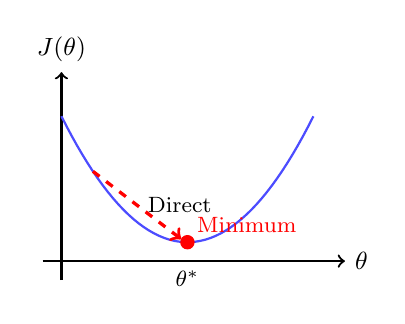
\begin{tikzpicture}[scale=0.8]
                % Axes
                \draw[->, thick] (-0.3,0) -- (4.5,0) node[right] {\small $\theta$};
                \draw[->, thick] (0,-0.3) -- (0,3) node[above] {\small $J(\theta)$};
                
                % Loss curve (parabola)
                \draw[thick, blue!70, domain=0:4, samples=50] plot (\x, {0.5*(\x-2)^2 + 0.3});
                
                % Direct arrow to minimum
                \draw[->, very thick, red, dashed] (0.5, {0.5*(0.5-2)^2 + 0.3}) -- (1.9, 0.35) node[midway, right, black] {\footnotesize Direct};
                
                % Minimum point
                \filldraw[red] (2, 0.3) circle (3pt);
                \node[below] at (2, 0) {\footnotesize $\theta^*$};
                \node[above right, red] at (2, 0.3) {\footnotesize Minimum};
            \end{tikzpicture}
            
            \vspace{0.8em}
            
            {\small 
            \textcolor{green!50!black}{\textbf{+}} Finds exact solution instantly\\
            \textcolor{red}{\textbf{$-$}} Only works for simple problems\\
            \textcolor{red}{\textbf{$-$}} Impossible for neural networks
            }
        \end{column}
        
        % --- Right: Gradient Descent ---
        \begin{column}{0.48\textwidth}
            \centering
            \textbf{Gradient Descent (Iterative)}
            
            \vspace{0.5em}
            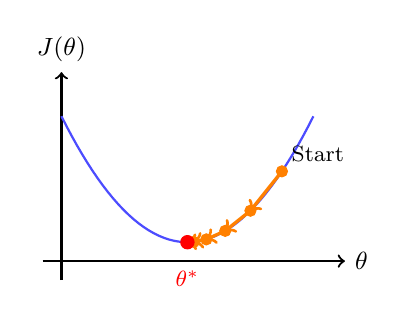
\begin{tikzpicture}[scale=0.8]
                % Axes
                \draw[->, thick] (-0.3,0) -- (4.5,0) node[right] {\small $\theta$};
                \draw[->, thick] (0,-0.3) -- (0,3) node[above] {\small $J(\theta)$};
                
                % Loss curve (parabola)
                \draw[thick, blue!70, domain=0:4, samples=50] plot (\x, {0.5*(\x-2)^2 + 0.3});
                
                % Iterative steps - calculated to be on the curve y = 0.5*(x-2)^2 + 0.3
                \coordinate (p0) at (3.5, {0.5*(3.5-2)^2 + 0.3});
                \coordinate (p1) at (3.0, {0.5*(3.0-2)^2 + 0.3});
                \coordinate (p2) at (2.6, {0.5*(2.6-2)^2 + 0.3});
                \coordinate (p3) at (2.3, {0.5*(2.3-2)^2 + 0.3});
                \coordinate (p4) at (2.1, {0.5*(2.1-2)^2 + 0.3});
                \coordinate (p5) at (2.0, {0.5*(2.0-2)^2 + 0.3});
                
                \filldraw[orange] (p0) circle (2.5pt);
                \draw[->, very thick, orange] (p0) -- (p1);
                \filldraw[orange] (p1) circle (2.5pt);
                \draw[->, very thick, orange] (p1) -- (p2);
                \filldraw[orange] (p2) circle (2.5pt);
                \draw[->, very thick, orange] (p2) -- (p3);
                \filldraw[orange] (p3) circle (2.5pt);
                \draw[->, very thick, orange] (p3) -- (p4);
                \filldraw[orange] (p4) circle (2.5pt);
                \draw[->, very thick, orange] (p4) -- (p5);
                \filldraw[red] (p5) circle (3pt);
                
                % Label
                \node[above right, black] at (p0) {\footnotesize Start};
                \node[below, red] at (2, 0) {\footnotesize $\theta^*$};
            \end{tikzpicture}
            
            \vspace{0.8em}
            
            {\small 
            \textcolor{green!50!black}{\textbf{+}} Works for any model\\
            \textcolor{green!50!black}{\textbf{+}} Universal for ML/DL\\
            \textcolor{orange!80!black}{\textbf{$-$}} Requires many iterations
            }
        \end{column}
    \end{columns}
    
    % \vspace{1em}
    % \centering
    % \small\textit{Update rule: } $\theta_{new} = \theta_{old} - \alpha \nabla J(\theta)$ \quad {\footnotesize($\alpha$ = learning rate)}
    
\end{frame}





\begin{frame}{How Gradient Descent Works}
    
    \textbf{Core Idea:} Move parameters in the direction that reduces loss.
    
    \vspace{1em}
    
    \begin{columns}[c]
        % Left: Visual
        \begin{column}{0.45\textwidth}
            \centering
            \begin{tikzpicture}[scale=1.1]
                % Axes
                \draw[->, thick] (-0.3,0) -- (4.5,0) node[right] {\small $\theta$};
                \draw[->, thick] (0,-0.3) -- (0,3.2) node[above] {\small $J(\theta)$};
                
                % Loss curve
                \draw[thick, blue!70, domain=0:4, samples=50] plot (\x, {0.5*(\x-2)^2 + 0.3});
                
                % Current point
                \coordinate (current) at (3.2, {0.5*(3.2-2)^2 + 0.3});
                \filldraw[black!80, fill=black!60] (current) circle (3.5pt);
                \node[right=3pt, black!80] at (current) {$\theta_t$};
                
                % % Tangent line (gradient)
                % \draw[orange, very thick, <->] (2.7, 1.1) -- (3.7, 1.9);
                % \node[above, orange] at (3.2, 1.7) {\footnotesize Slope = $\nabla J(\theta_t)$};
                
                % Arrow showing update direction
                \draw[->, !60!black, line width=2pt]
                (current) -- ++(-0.6, -0.5)
                node[left=15pt, above=8pt, font=\footnotesize] {$-\alpha \nabla J$};

                
                % Next point
                \coordinate (next) at (2.5, {0.5*(2.5-2)^2 + 0.3});
                \filldraw[red!60!black, fill=red!40] (next) circle (3.5pt);
                \node[below, red!60!black] at (next) {$\theta_{t+1}$};
            \end{tikzpicture}
        \end{column}
        
        % Right: Steps
        \begin{column}{0.5\textwidth}
            \textbf{Step-by-Step Process:}
            
            \vspace{0.5em}
            
            \begin{enumerate}
                \item \textbf{Compute Loss}\\
                {\small Evaluate $J(\theta_t)$ at current parameters}
                
                \vspace{0.3em}
                
                \item \textbf{Calculate Gradient}\\
                {\small Find slope: $\nabla J(\theta_t) = \frac{\partial J}{\partial \theta}$}
                
                \vspace{0.3em}
                
                \item \textbf{Update Parameters}\\
                {\small Move opposite to gradient with a step size (learning rate) $\alpha$:}
                $$\theta_{t+1} = \theta_t - \alpha \nabla J(\theta_t)$$
                
                % \vspace{0.3em}
                
                \item \textbf{Repeat}\\
                {\small Until convergence (loss stops decreasing)}
            \end{enumerate}

        \end{column}
    \end{columns}
    
\end{frame}


\subsection{The Learning Loop}

\begin{frame}{Putting It All Together: The Learning Loop}
    \centering
    
    \vspace{0.25em}
    
    \begin{tikzpicture}[
        node distance=2.0cm,
        auto,
        thick,
        % Styles for the blocks
        block/.style={
            rectangle, 
            draw, 
            rounded corners=5pt,
            text width=2.4cm, 
            text centered, 
            minimum height=1.1cm,
            font=\small\bfseries,
            line width=1.1pt
        },
        line/.style={draw, -{Latex[length=2.3mm]}, line width=1.1pt}
    ]
        % --- Nodes ---
        % 1. Data (left)
        \node [block, fill=gray!20] (data) {Data\\$(x, y)$};
        
        % 2. Model (center)
        \node [block, fill=blue!20, right=1.3cm of data] (model) {Model\\$\hat{y} = f_\theta(x)$};
        
        % 3. Loss (right)
        \node [block, fill=red!20, right=1.9cm of model] (loss) {Loss Function\\$J(\theta)$};
        
        % 4. Optimizer (below model)
        \node [block, fill=green!20, below=1.0cm of model] (opt) {Optimizer};
        
        % --- Flows ---
        % Data -> Model (input x)
        \path [line, blue!70] (data) -- node [below, black] {\scriptsize Input $x$} (model);
        
        % Data -> Loss (true labels y)
        \path [line, gray!70] (data.north) to[bend left=15] node [above, black, pos=0.5] {\scriptsize True $y$} (loss.north);
        
        % Model -> Loss (predictions)
        \path [line, red!70] (model) -- node [below, black] {\scriptsize Predictions $\hat{y}$} (loss);
        
        % Loss -> Optimizer (gradients)
        \path [line, orange!70] (loss.south) to[bend left=20] node [left, black, pos=0.3] {\scriptsize Compute $\nabla J$} (opt.east);
        
        % Optimizer -> Model (update weights)
        \path [line, green!70] (opt) -- node [left, black] {\scriptsize Update $\theta$} (model);
        
    \end{tikzpicture}
    
    \vspace{0.5em}
    
    \begin{columns}[T]
        \begin{column}{0.48\textwidth}
            \textbf{Forward Pass:}
            \begin{itemize}
                \item Data $\to$ Model $\to$ Predictions
                \item Compute Loss
            \end{itemize}
        \end{column}
        
        \begin{column}{0.48\textwidth}
            \textbf{Backward Pass:}
            \begin{itemize}
                \item Calculate gradients
                \item Update parameters
            \end{itemize}
        \end{column}
    \end{columns}
    
    \vspace{0.25em}
    \centering
    \textit{Repeat until loss converges (model learns)!}
    
\end{frame}








% =========================
% 3. Main Challenges
% =========================

\section{Main Challenges of Machine Learning}
